\header{
    \headtitle{Sa Grande Pine} \label{sa-grande-pine}
    %
    \insertComment{}{}
}

\enluminure{4}{\href{https://www.youtube.com/watch?v=j1zHxnIb1cE}{J}}{'étais} pucelle et ce soir-là,
\\Dans le jardin, sous les glycines,
\\Mon premier béguin me montra
\\Sa Grande Pine
\\Puis, fourrageant sous mon jupon,
\\Sa forte main se fit câline,
\\Et je sentis dans un frisson
\\Sa Grande Pine
\\\\D'abord je criai de douleur,
\\Mais dans sa rage qui s'obstine
\\Elle m'enseigna le bonheur
\\Sa Grande Pine
\\Et labourée par ses assauts,
\\Je gémis la plainte divine
\\Que m'arracha dans ses sursauts
\\Sa Grande Pine
\\\\Tout me devint indifférent,
\\Succès, richesse ou bien débine,
\\Lorsque je sentis dans mes flancs
\\Sa Grande Pine
\\Depuis je ne crains plus, ma foi,
\\Tout ce que le sort me destine,
\\Pourvu que bande auprès de moi
\\Sa Grande Pine
\\\\Elle s'égare quelquefois
\\Dans ma bouche rendue coquine,
\\Ou bien se meurt entre mes doigts,
\\Sa Grande Pine
\\Ou bien, sur un rythme insensé,
\\Rêvant d'un gars de la marine,
\\Elle se trompe de coté,
\\Sa Grande Pine
\breakpage
Qu'aux années s'ajoutent les ans,
\\Que lassitude se devine,
\\Je ne veux mourir qu'en serrant
\\Sa Grande Pine
\\Et plutôt que le Paradis,
\\Mieux vaux l'Enfer où se dessine,
\\Dans l'ombre des plaisirs maudits,
\\Sa Grande Pine
\begin{center}
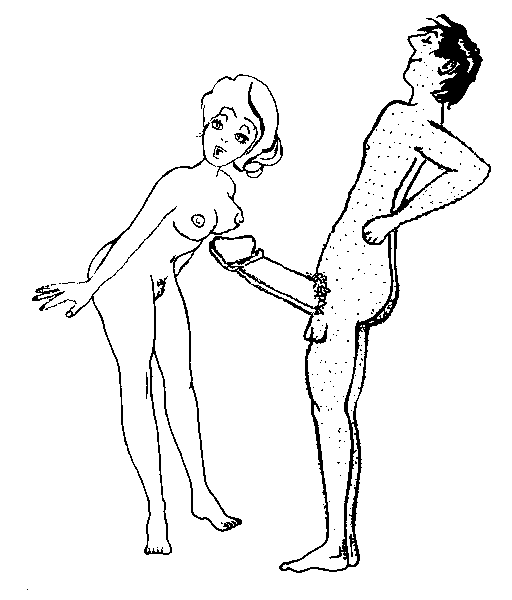
\includegraphics[width=1\textwidth]{images/grande_pine.png}
\end{center}

\breakpage